\documentclass{thesis-ekf}
\usepackage[T1]{fontenc}
\PassOptionsToPackage{defaults=hu-min}{magyar.ldf}
\usepackage[magyar]{babel}
\usepackage{mathtools,amssymb,amsthm,pdfpages}
\footnotestyle{rule=fourth}

\newtheorem{tetel}{Tétel}[chapter]
\theoremstyle{definition}
\newtheorem{definicio}[tetel]{Definíció}
\theoremstyle{remark}
\newtheorem{megjegyzes}[tetel]{Megjegyzés}

\usepackage{listings}
\usepackage{array}
\setlength{\extrarowheight}{2pt}

\begin{document}

\institute{Matematikai és Informatikai Intézet}
\title{\LaTeX beadandó}
\author{Zana Domán\\Programtervező informatikus}
\supervisor{Hekk Elek\\Tanársegéd}
\city{Eger}
\date{2025}
\maketitle

\tableofcontents

\chapter{Doom (videójáték, 1993)}

\section{A játék bemutatása}

A Doom (magyarul \textqq{Végzet}) \footnote{A játék címét \textit{A pénz színe}
című film egyik jenelete inspirálta.} Belső nézetű lövöldözős játék, amelyet
1993-ban adott ki az id Software MS-DOS operációs rendszerre. A játékos a
Doomguy becenevet viselő katonát irányítja, akinek megfertőzött zombikat és
pokolból szabadult démonokat kell legyőznie. Az első fejezet shareware formában
terjedt, a teljes játékot 2 további fejezettel kiegészítve lehetett megvásárolni
az id Software-től postán keresztül. A játék frissített változata boltokban is
megjelent Ultimate Doom néven, amely egy újabb, negyedik fejezetet is
tartalmazott. Folytatása, a Doom II: Hell on Earth 1994-ben jelent meg.

\begin{figure}[h]
    \centering
    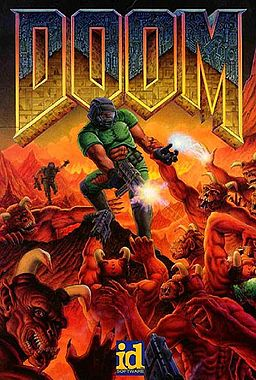
\includegraphics[width=5cm]{doom.jpg}
\end{figure}

A Doom az egyik legfontosabb játék a videójátékok történelmében, gyakran említik
a valaha volt legjobb és legfontosabb játékként, technikai újításai nagy
hatással voltak a 3D, belső nézetű, illetve többszemélyes játékokra. Világszerte
3.5 millió darabot adtak el, és több mint 10 és 20 millió közötti ember
játszotta a megjelenése utáni első két évben, becslések szerint több gépre volt
feltelepítve, mint a Microsoft akkori új operációs rendszere, a Windows 95. A
nagy sikernek és technikai újításainak köszönhetően rengeteg más fejlesztő
használta a játék motorját saját játékukhoz, vagy ahhoz hasonló motort
készítettek, ezeket Doom klónoknak hívják, amelyek közül a legismertebb a Duke
Nukem 3D. A játékot könnyen lehet módosítani a WAD fájlban tárolt adatok
átszerkesztésével. A játék véres, erőszakos és pokoli ábrázolásai viták tárgyát
képezték, és egyike volt azon játékoknak, amely miatt az ESRB korhatár besorolás
létrejött.

\section{A játék menete}

Stílusát tekintve belső nézetű lövöldözős játék, ahol a cél, hogy a játékos a
rendelkezésre álló fegyvereivel legyőzze a számítógép által vezérelt
ellenségeket. A játék fejezetekre van bontva, egy fejezeten belül 9 szint
található, amelyből egy titkos. A következő szintre az adott szint végének
elérésével lehet eljutni, amely általában egy liftben található kapcsoló, vagy
egy teleport kapu. A szinteken titkos helyek is előfordulnak, amelyek
eljutásához a játékosnak meg kell keresni az ahhoz vezető bejáratot, ez lehet
egy más színezésű fal, vagy egy rejtett kapcsoló által kinyitott ajtó, illetve
ezeken keresztül lehet titkos szintekre is eljutni. Előfordulnak továbbá
elszórva felvehető tárgyak, mint pl. elsősegély doboz, lőszer, fegyver, kulcsok
amelyekkel lezárt ajtókat tud a játékos kinyitni a tovább haladáshoz, vagy
titkos részeken található gömbök, amelyek egy extra képességgel ruházzák fel a
játékost (pl. sebezhetetlenség, láthatatlanság), továbbá az ellenségek,
kapcsolók, ajtók, lépcsők, liftek, hullák és robbanásveszélyes hordók.

\section{A játék tartalma}

\subsection{Fegyverek}

A játékban nyolc fegyvert használhat a játékos:

\begin{itemize}
    \item \textbf{Ököl}: alap fegyver, nem használ lőszert.
    \item \textbf{Láncfűrész}: lecseréli az ököl fegyvert ha a játékos felveszi,
        nem használ lőszert.
    \item \textbf{Pisztoly}: alap fegyver, tölténytárat használ lőszerként.
    \item \textbf{Sörétes puska}: egycsövű sörétes puska, sörétes lőszert
        használ lőszerként.
    \item \textbf{Golyószóró}: Gatling-típusú forgótáras gépfegyver,
        tölténytárat használ lőszerként.
    \item \textbf{Rakétavető}: vállról indítható rakétavető, rakétákat használ
        lőszerként.
    \item \textbf{Plazma puska}: gyorstüzelésű plazmafegyver, plazma cellákat
        használ lőszerként.
    \item \textbf{BFG 9000}: teljes nevén: „Big Fucking Gun 9000”, magyarul:
        „Kibaszott Nagy Fegyver 9000”, nagy teljesítményű plazmafegyver, plazma
        cellákat használ lőszerként.
\end{itemize}

\subsection{Ellenségek}

A játékban tíz ellenség található:

\begin{itemize}
    \item \textbf{Zombieman}: Zombivá változott katona, a játék leggyakrabban
        előforduló, illetve leggyengébb ellensége, miután meghal egy
        tölténytárat dob el.
    \item \textbf{Shotgun guy}: Sörétes puskával rendelkező zombikatona, a
        Zombieman mellett a leggyakrabban előforduló ellenség, miután meghal
        egy sörétes puskát dob el.
    \item \textbf{Imp}: Barnaszínű, izmos, emberalkatú démon, testéből tüskék
        állnak ki, tűzlabdák dobálásával vagy karmolással támad.
    \item \textbf{Pinky Demon}: Rózsaszín, tömzsi, izmos testalkatú de
        emberméretű démon, harapással támad, a leggyorsabb ellenség a játékban.
    \item \textbf{Spectre}: A Demon láthatatlan változata.
    \item \textbf{Cacodemon}: Piros színű, gömbölyű, repülő démon, tűzlabdák
        lövésével vagy harapással támad. Nem jelenik meg az első fejezetben.
    \item \textbf{Lost Soul}: Repülő, tűzben lángoló koponya szarvakkal, a
        játékosnak nekirepülve harapással támad. Nem jelenik meg az első
        fejezetben.
    \item \textbf{Baron of Hell}: Rózsaszín, magas és izmos testalkatú démon,
        zöld plazmák dobálásával vagy karmolással támad.
    \item \textbf{Cyberdemon}: A második fejezet főgonosza, egy emberalkatú,
        bőrszínű, magas és izmos testalkatú démon pár mechanikus végtaggal,
        rakéták kilövésével támad. Nem jelenik meg az első fejezetben.
    \item \textbf{Spider Mastermind}: A harmadik fejezet egyben a játék
        főgonosza, egy pókalkatú, mechanikus végtagokkal rendelkező agy
        kinézetű démon, golyószóróval támad. Nem jelenik meg az első fejezetben.
\end{itemize}

\chapter{Doom technikai megvalósítása}

\section{A játék motorja}

A Doom-motor \footnote{A Doom-motor, később bevezetett számozással id Tech 1.
néven vált ismertté.} technikailag nagy előrelépésnek számított megjelenésekor.
A fejlesztők egyaránt törekedtek a minél szebb látványvilág megjelenítésére és a
gépigény alacsony szinten tartására. Mivel az akkori hardvereken túl lassú lett
volna egy valódi, teljesen 3D megjelenítés, ál-3D grafikát kapott a játék.

Az id Software előző játékához, a Wolfenstein 3D-hez képest több újítás került a
motorba. Megjelentek a magassági különbségek: míg a Wolfenstein 3D-ben minden
padló és plafon sík volt, a Doom-ban tetszőlegesen változhatott a magasságuk. A
Doom szakított az előd labirintus-jellegével is, pályatervezéskor nem szükséges
már derékszögűnek lennie a falak csatlakozásának, ezenkívül megjelentek a
külterek is a pályákon. Futás vagy gyaloglás közben a fegyver himbálózása
mozgásérzetet kelt a játékosban: a Wolfenstein 3D-ben a főszereplő karjai nem
mozognak. Teljes a textúrázottság minden felületen, szemben a Wolfenstein 3D
textúra nélküli padlójával és plafonjával. A pályákon megjelenik az
interaktivitás: a platformok akár le és föl tudnak mozogni, csakúgy mint a
padlók és a hidak, melyek szintén felemelkedhetnek és lesüllyedhetnek. A Doomban
a fényviszonyok is változnak, az árnyékok és fényforrások hozzájárultak a játék
látványvilágának hitelesebbé tételéhez. A valós életérzetet továbbá a sztereó
hangzás is elősegítette, amelyből következtetni lehetett nagyjából, hogy honnan
és milyen távolságból jöhetnek a hangok. Például a játékos figyelmét
felkelthetik a szörnyek röfögései és morgásai, mert hallhatja, hogy honnan
számíthat ellenségre. Az ajtók nyitódását és záródását is meghallhatja, ezáltal
rátalálhat különböző titkos rejtekhelyekre.

A Doom pályái nem teljesen háromdimenziósak, mert belülről egy síkon vannak
ábrázolva (ez látható a játék beépített térképén), a terek falakkal és
magassági különbségekkel voltak elválasztva. A mai, 3D vertexekre épülő
geometriával szemben több megkötés is van: például nem lehet két szoba egymás
fölött, nem lehet tetszőleges szögben szétnézni a fellépő nagy torzulások miatt.
Előnye viszont a gyorsaság, amit BSP (Binary Space Partitioning, bináris
térfelosztás) alapú rendereléssel ér el, továbbá előnyös a 2D pályaábrázolás a
beépített térkép rajzolásakor is.

Fontos újítás a motorban a moduláris megközelítés, ami megengedi a játék
tartalmának lecserélését a WAD adatfájlok cseréjével (lásd lentebb). Az előd
Wolfenstein 3D-ben nem volt meg ez a lehetőség, bár a játék fanatikusai
rájöttek, hogyan tudnak saját pályákat készíteni. A Doom ezzel szemben megadta a
lehetőséget, ami jelentősen növelte a népszerűségét.

\section{A játék pályáinak felépítése}

A Doom összes pályája 2D-s. Ezt jól mutatja az is, hogy a pályákon nem lehet két
szektort elhelyezni egymás fölé vagy alá. Azonban ennek a korlátnak van egy
előnye is, mégpedig a térkép megjelenítése, amely megmutatja, hogy éppen hol áll
a játékos a pályán.

\subsection{Alapvető objektumok}

Az alapvető egység a \textqq{vertex}, vagyis a csúcspont, amely egy egyszerű
2D-s pontot ábrázol. A csúcspontok a line-okba, azaz a vonalakba kapcsolódnak,
amelyeket \textqq{linedefs}-nek nevezünk. Minden egyes linedefs-nek van egy vagy
két oldala, amelyeket \textqq{sidedefs}-nek nevezünk. Ha a sidedefs-eket
csoportba foglaljuk, akkor \textqq{polygon}-okat, azaz sokszögeket alkotnak,
amelyeket csoportos nevükön szektoroknak hívunk. A szektorok képviselik a pálya
részletes területeit.

\subsection{Szektorok}

Minden egyes szektornak négy tulajdonsága van: a padló magassága, a plafon
magassága, a szektor fényereje, illetve a padló és a plafon mintája. Több
különböző világosságú szektor létrehozásához, különböző fényerejű szektorokat
kell létrehozni. Ezért van az, hogy amíg egy egyoldalas linedef egy térbeli
\textqq{falnak} látszódik, addig a szektorok között egy kétoldalas linedef egy
\textqq{hídnak} látszódik.

\subsection{Sidedefek}

A sidedefek tartalmazzák a falak textúráját: ezek teljesen elkülönülnek a padló
és a plafon textúráitól. Minden egyes sidedefnek három textúrája van, amelyeket
középső, felső és alsó textúráknak hívunk. Egy egyoldalú linedef csak egy
középső textúrát használhat egy fal textúrázásához. Egy kétoldalú linedefnek egy
kicsit összetettebb a textúrázási folyamata. Az alsó és a felső textúrák azokra
a helyekre kerülnek fel, ahol a két szektor között szintkülönbség van (például
egy lépcső, amelyre alsó textúra kerül). Egy sidedefnek szintén egy középső
textúrája van, bár nem mindig: mivel ez felel a függő textúrákért is, mint
például az égboltért.

\section{További Doom-motort használó játékok}

\begin{itemize}
    \item id Software
        \begin{itemize}
            \item 1993
                \begin{itemize}
                    \item Doom
                \end{itemize}
            \item 1994
                \begin{itemize}
                    \item Doom II: Hell on Earth
                \end{itemize}
            \item 1995
                \begin{itemize}
                    \item The Ultimate Doom
                    \item Master Levels for Doom II
                \end{itemize}
        \end{itemize}
    \item Raven Software
        \begin{itemize}
            \item 1994
                \begin{itemize}
                    \item Heretic
                \end{itemize}
            \item 1995
                \begin{itemize}
                    \item Hexen: Beyond Heretic
                \end{itemize}
            \item 1996
                \begin{itemize}
                    \item Heretic: Shadow of the Serpent Riders
                    \item Hexen: Deathkings of the Dark Citadel
                \end{itemize}
        \end{itemize}
    \item TeamTNT
        \begin{itemize}
            \item 1996
                \begin{itemize}
                    \item Final Doom
                \end{itemize}
        \end{itemize}
    \item Rogue Entertainment
        \begin{itemize}
            \item 1996
                \begin{itemize}
                    \item Strif: Quest for the Sigil
                \end{itemize}
        \end{itemize}
\end{itemize}

\chapter{Extra feladatok}

\section{Programkód}

\lstinputlisting[numbers=left,language=C,label={lst:reverse}]{reverse.c}
\Aref{lst:reverse} programkód rekurzió segítségével fordít meg egy
karakterláncot.

\section{Táblázat}

\begin{table}[h]
    \centering
    \footnotesize
    \begin{tabular}{|>{\bfseries}l|l|l|l|l|l|}
        \cline{2-6}
        \multicolumn{1}{c|}{} & \multicolumn{5}{c|}{\textbf{Órarend}}\\
        \cline{2-6}
        \multicolumn{1}{c|}{} &
        \multicolumn{1}{c|}{\textbf{Hétfő}} &
        \multicolumn{1}{c|}{\textbf{Kedd}} &
        \multicolumn{1}{c|}{\textbf{Szerda}} &
        \multicolumn{1}{c|}{\textbf{Csütörtök}} &
        \multicolumn{1}{c|}{\textbf{Péntek}} \\
        \hline
        08.00--08.45 &
        matematika &
        rajz &
        irodalom &
        angol &
        matematika\\
        \hline
        08.55--09.40 &
        ének-zene &
        testnevelés &
        matematika &
        kémia &
        történelem\\
        \hline
        09.50--10.35 &
        irodalom &
        matematika &
        angol &
        matematika &
        testnevelés\\
        \hline
        10.45--11.30 &
        nyelvtan &
        történelem &
        biológia &
        nyelvtan &
        angol\\
        \hline
    \end{tabular}
\end{table}

\begin{thebibliography}{2}
\addcontentsline{toc}{chapter}{\bibname}
\end{thebibliography}

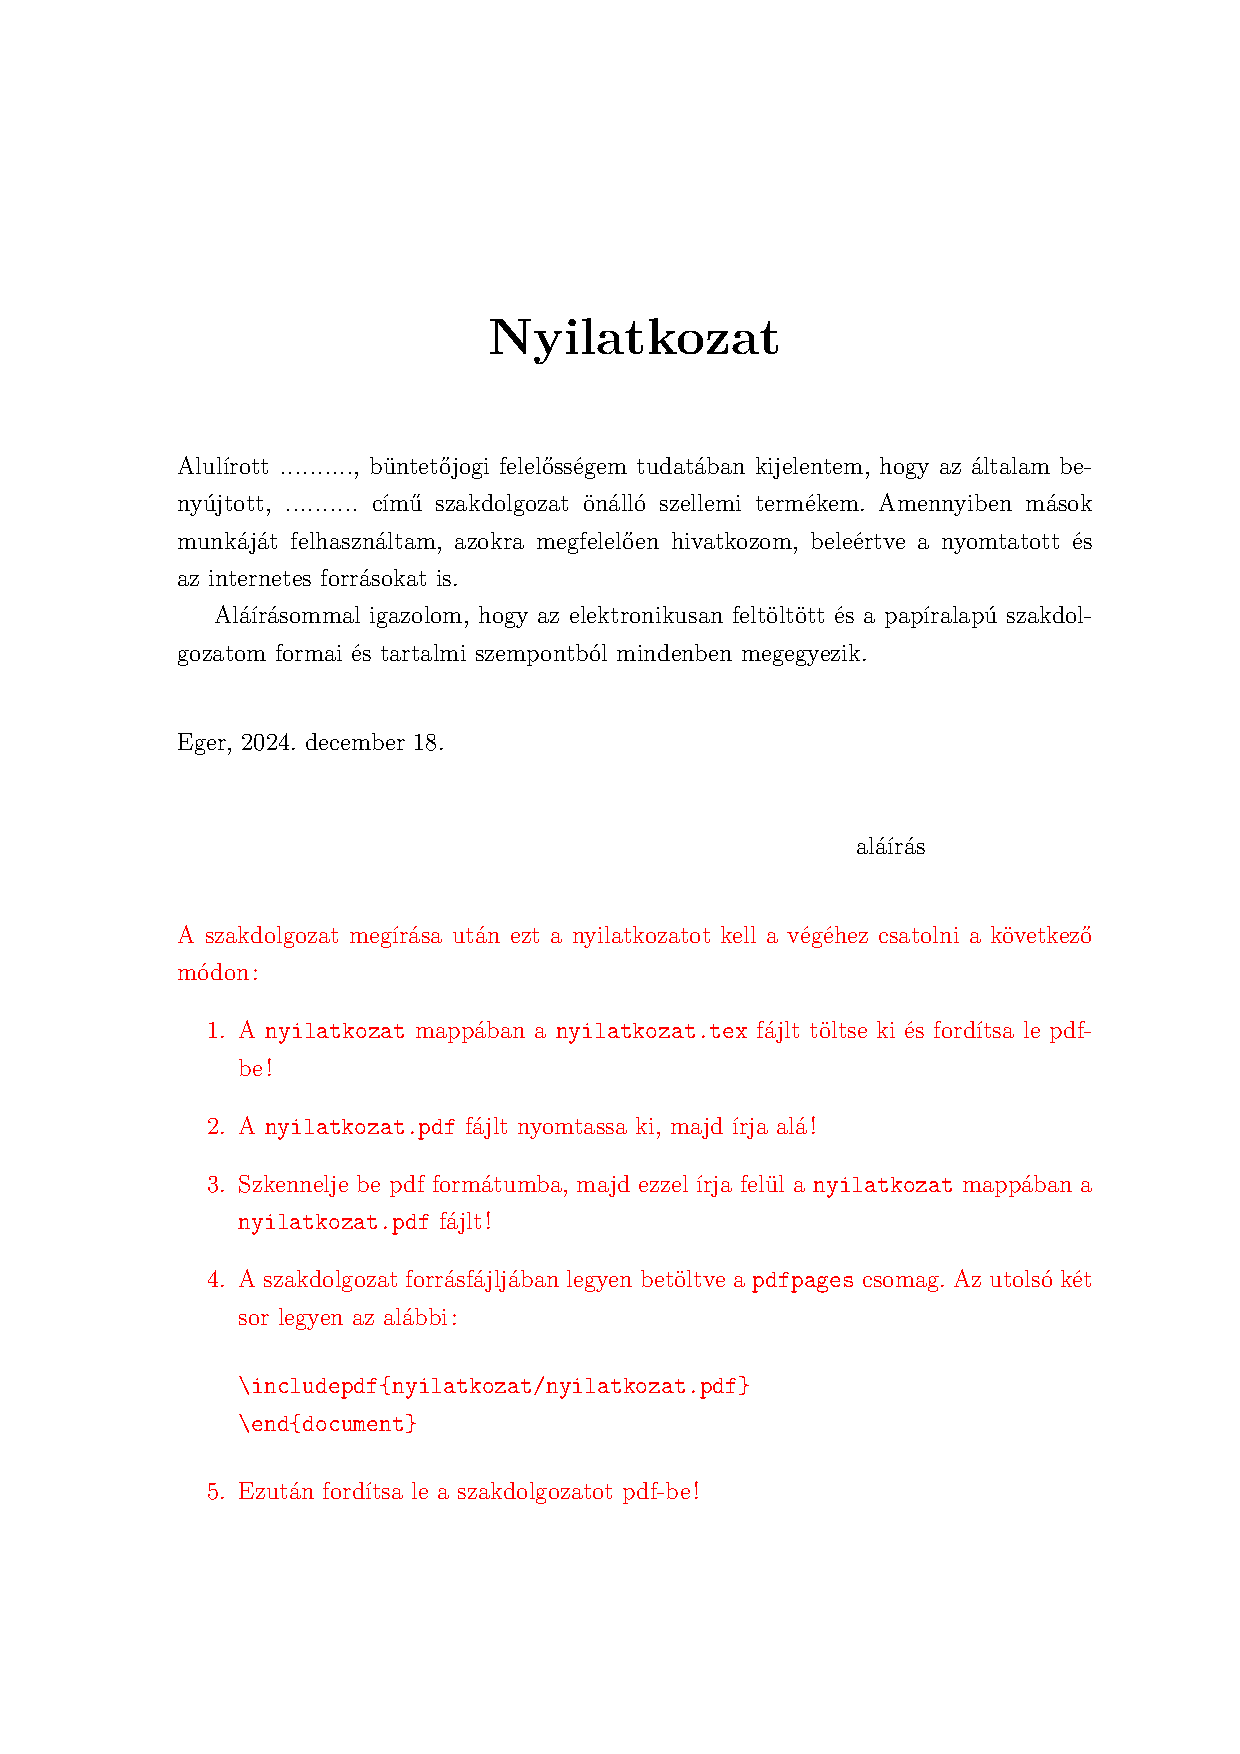
\includepdf{nyilatkozat/nyilatkozat.pdf}
\end{document}
